\documentclass{beamer}
%
% Choose how your presentation looks.
%
% For more themes, color themes and font themes, see:
% http://deic.uab.es/~iblanes/beamer_gallery/index_by_theme.html
%
\mode<presentation>
{
  \usetheme{default}      % or try Darmstadt, Madrid, Warsaw, ...
  \usecolortheme{crane} % or try albatross, beaver, crane, ...
  \usefonttheme{structurebold}  % or try serif, structurebold, ...
  \setbeamertemplate{navigation symbols}{}
  \setbeamertemplate{caption}[numbered]
} 

%\setbeamertemplate{footline}[page number]

\usepackage[utf8]{inputenc}

\usepackage{amsmath}

\usepackage{amssymb}
\usepackage{amsthm}
\usepackage{color}
\usepackage{comment}

\usepackage{hyperref}

\usepackage{tikz}
\usetikzlibrary{quantikz}

\renewcommand{\>}{\rangle}
\newcommand{\<}{\langle}

\newcommand{\calE}{\mathcal{E}}
\newcommand{\calL}{\mathcal{L}}

\newcommand{\cS}{\mathcal{S}}

\newcommand{\C}{\mathbb{C}}
\newcommand{\R}{\mathbb{R}}

\newcommand{\tr}{\mathrm{tr}}

\newcommand{\cH}{\mathcal{H}}
\newcommand{\B}{\mathbb{B}}

\newcommand{\cC}{\mathcal{C}}
\newcommand{\cE}{\mathcal{E}}
\newcommand{\cF}{\mathcal{F}}
\newcommand{\cG}{\mathcal{G}}
\newcommand{\cT}{\mathcal{T}}
\newcommand{\cL}{\mathcal{L}}
\newcommand{\cM}{\mathcal{M}}
\newcommand{\cO}{\mathcal{O}}
\newcommand{\cR}{\mathcal{R}}
\newcommand{\cV}{\mathcal{V}}
\newcommand{\cU}{\mathcal{U}}
\newcommand{\cX}{\mathcal{X}}

\newcommand{\fA}{\mathfrak{A}}
\newcommand{\fB}{\mathfrak{B}}
\newcommand{\fC}{\mathfrak{C}}

\newcommand{\fix}{\mathrm{Fix}}

\newcommand{\avg}{\mathrm{avg}}

\newcommand{\cW}{\mathcal{W}}

\newcommand{\tg}{\tilde{g}}
\newcommand{\tU}{\tilde{U}}
\newcommand{\tV}{\tilde{V}}

\newcommand{\Clim}{\mathfrak{C}}

\usetikzlibrary{shadows.blur}

\definecolor{neongreen}{RGB}{0, 255, 128}
\definecolor{neonpink}{RGB}{255, 20, 147}
\definecolor{neonblue}{RGB}{0, 255, 255}
\definecolor{neonyellow}{RGB}{255, 255, 102}
\definecolor{neonpurple}{RGB}{180, 0, 255}
\definecolor{neongrid}{RGB}{255, 0, 255}
\definecolor{spaceblack}{RGB}{10,10,30}
\definecolor{gridcolor}{RGB}{255, 109, 194}

%%

\title{Quantized Markov chain couplings that prepare Qsamples}
\author{Pawe{\l} Wocjan}
\institute{Quantum Algorithms Group, IBM Quantum} %\\ IBM T.~J.~Watson Research Center}
%\date{Keio University\\November 12, 2025}
\date{Institute for Pure \& Applied Mathematics\\
University of California, Los Angeles\\
January 14, 2026}
\begin{document}

\begin{frame}
  \titlepage
\end{frame}

%%

\begin{frame}{Based on}

    \emph{Quantized Markov chain couplings that prepare Qsamples}

    \medskip
    Kristan Temme and Pawel Wocjan

    \medskip
    Quantum 9, 1951 (2025), \url{https://arxiv.org/abs/2504.02651}
\end{frame}

%%

%%%%%%%%%%%%%%%%%%%%%%%%%%%%%%%%%%%%%%%%%%%%%%%%%%%%%%%%%%%%%%%%%%%%%%%%%%%%%%%

\begin{frame}{Quantum algorithms}

\medskip
With steady progress in quantum hardware, error correction, and fault tolerance,

\bigskip
\textbf{the search for new quantum algorithms for large-scale fault-tolerant quantum computers has become more critical than ever.}

\end{frame}

%%

\begin{frame}{Galactic Scale Research Description}

\begin{center}
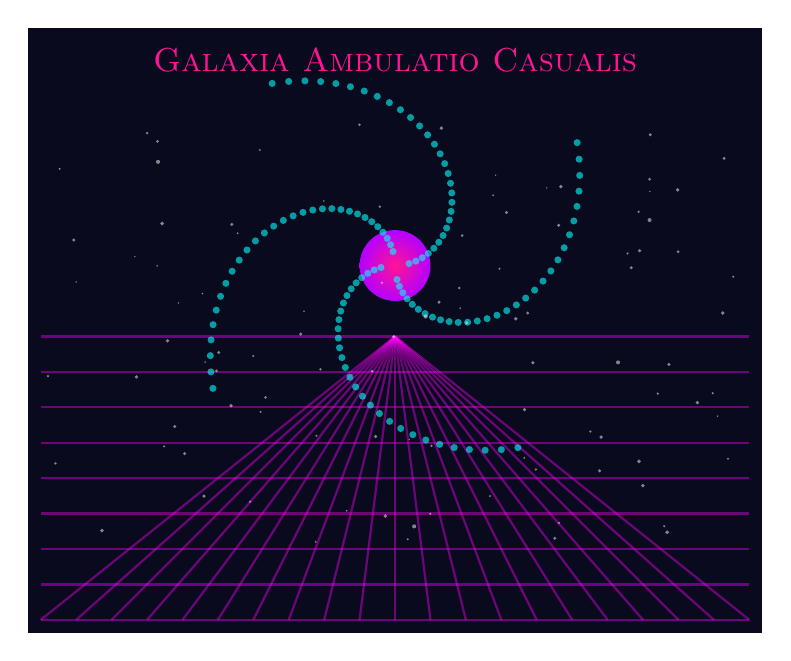
\begin{tikzpicture}[scale=0.9, background rectangle/.style={fill=spaceblack}, show background rectangle]

% Grid horizon
\begin{scope}[shift={(-5,-4)}]
  \foreach \x in {0,0.5,...,10} {
    \draw[neongrid, opacity=0.4, thick] (\x,0) -- (5,4);
  }
  \foreach \y in {0,0.5,...,4} {
    \draw[neongrid, opacity=0.4, thick] (0,\y) -- (10,\y);
  }
\end{scope}


% Galactic core with glow
\shade[inner color=neonpink, outer color=neonpurple] (0,1) circle (0.5);

% Spiral arms (simplified)
\foreach \angle in {0,90,180,270} {
  \foreach \r in {0.2, 0.3,...,3.2} {
    \pgfmathsetmacro{\x}{\r * cos(\angle + 40 * \r)}
    \pgfmathsetmacro{\y}{1 + \r * sin(\angle + 40 * \r)}
    \fill[neonblue, opacity=0.6] (\x,\y) circle (0.05);
  }
}

% Background stars
\foreach \i in {1,...,100} {
  \pgfmathsetmacro{\x}{rnd*10 - 5}
  \pgfmathsetmacro{\y}{rnd*6 - 3}
  \fill[white, opacity=0.5] (\x,\y) circle (0.01 + rnd*0.02);
}

% Adding the name "Galaxia Markovus"
\node[neonpink, above] at (0,3.6) {\large \textsc{Galaxia Ambulatio Casualis}};

\end{tikzpicture}
\end{center}
\end{frame}

%%

\begin{frame}{Sampling from probability distributions}
\begin{itemize}
    \item Many important problems in computer science, physics, and machine learning can be solved by sampling from interesting probability distributions.

    \medskip
    \item Markov chains are an important algorithmic tool for efficiently generating such samples.

    \bigskip
    \item For instance, one application is approximating the best route for the traveling salesman problem using simulated annealing, which employs a Markov chain parameterized by temperature.

    \medskip
    \item Well-designed Markov chains enable us to cleverly explore exponentially large state spaces.
\end{itemize}
\end{frame}

%%

\begin{frame}{Qsamples -- quantum encodings of probability distributions}

\begin{itemize}
    \item Let $\pi=(\pi_x : x \in \Omega)$ be a probability distribution over a finite state space $\Omega$.
    
    \medskip
    \item The qsample $|\sqrt{\pi}\>$ is a quantum state encoding the classical state $\pi$.
    
    \medskip
    \item It is given by
    \begin{align*}
        |\sqrt{\pi}\> 
        &=
        \sum_{x\in\Omega} \sqrt{\pi_x} |x\>.
    \end{align*}

    \item Quantum algorithms leverage qsamples to achieve speed-ups.
\end{itemize}
\end{frame}

%%

\begin{frame}{Examples of applications of qsamples I}

\begin{itemize}
    \item Preparing a uniform superposition $|G\>$ over all group elements of a finite group $G$
    \begin{align*}
        |G\> 
        &= 
        \frac{1}{\sqrt{|G|}} \sum_{g\in G} |g\>
    \end{align*}
    is the first step in quantum algorithms for solving the hidden subgroup problem (e.g., Shor's DLOG quantum algorithm).
\end{itemize}
    
\end{frame}

%%

\begin{frame}{Examples of applications of qsamples II}

\begin{itemize}
    \item Decoded Quantum Interferometry prepares a qsample -- a purification -- of the density matrix
    \begin{align*}
        \sigma &= \frac{\mathcal{P}^2(H)}{\mathrm{Tr}(\mathcal{P}^2\big(H)\big)}
    \end{align*}
    for a Hamiltonian $H$ and a polynomial $\mathcal{P}$.

    \bigskip
    \item 
    The qsample has the form
    \begin{align*}
        (\sqrt{\sigma} \otimes I) |\Phi\>
    \end{align*}
    where $|\Phi\>$ is the (unormalized) maximally entangled state.
\end{itemize}
    
\end{frame}

%%

\begin{frame}{Examples of applications of qsamples III}

\begin{itemize}
    \item A quantum sample $|\sqrt{\pi}\>$ is a crucial ingredient for the quantum Chebyshev method, which enables one to reduce the cost from $O(1/\varepsilon^2)$ to $O(1/\varepsilon)$ when estimating the mean of a random variable with relative error $\varepsilon$.

    \bigskip

    \bigskip
    \item A quantum sample $|\sqrt{\pi}\>$ is key to obtaining speed-ups in other applications, such as finding marked elements, testing properties of distributions etc.

\end{itemize}
    
\end{frame}

%% 

\begin{frame}{Comments on the hardness of preparing qsamples}

\begin{itemize}
    \item Preparing qsamples of general probability distributions is very hard.

    \medskip
    \item Problems in SZK (Statistical Zero Knowledge) could be solved on quantum computers with the help of qsamples of probability distributions that are generated by classical circuits.
    
    \bigskip
    \item Preparing qsamples of stationary distribution for general Markov chains is very difficult.

    \medskip
    \item For instance, one could solve graph isomorphism with the help of the uniform superposition of all graphs isomorphic to a given graph.
\end{itemize}
    
\end{frame}

%%

\begin{frame}{Markov chain terminology I}
\begin{itemize}
    \item Let $P=(p_{x',x})$ denote the transition matrix of an ergodic Markov chain on state space $\Omega$ with stationary distribution $\pi=(\pi_x)$.

    \medskip
    \item For any initial probability distribution $q$, we have
    \begin{align*}
        \lim_{m\rightarrow\infty} P^m q = \pi.
    \end{align*}
\end{itemize}
\end{frame}

%%

\begin{frame}{Markov chain terminology II}
\begin{itemize}
    \item Define 
\begin{align*}
    d(m) 
    &=
    \max_{x\in\Omega} \, \frac{1}{2} \sum_{x'\in\Omega} 
    \big| [P^m]_{x',x} - \pi_{x'} \big|,
\end{align*}
where 
\begin{align*}
    ([P^m]_{x',x} : x' \in\Omega)
\end{align*} 
is the probability distribution that we obtain by starting the Markov chain in the initial state $x$ and making $m$ transitions.

\bigskip
\item The total variation distance $d(m)$ measures how close we are to the desired stationary distribution $\pi$ as the number of steps $m$ increases. 
\end{itemize}
\end{frame}

%%

\begin{frame}{Markov chain terminology III}
\begin{itemize}
\item The mixing time $t_\mathrm{mix}(\varepsilon)$ is defined by
\begin{align*}
    t_\mathrm{mix}(\varepsilon) 
    &= 
    \min\{m : d(m) \le \varepsilon \}
\end{align*}
for $\varepsilon\in (0,1)$. 

\bigskip
\item It satisfies the bound
\begin{align*}
    t_\mathrm{mix}(\varepsilon) 
    &\le \big\lceil \log_2\varepsilon^{-1} \big\rceil t_\mathrm{mix},
\end{align*}
where $t_\mathrm{mix}=t_\mathrm{mix}(1/4)$.
\end{itemize}
\end{frame}

%%

\begin{frame}{Galactic Scale Research Summary I}

\begin{itemize}
    \item Given a certain Markov chain $P$ with stationary distribution $\pi$, we construct an efficiently implementable quantum channel $\cT$ such that
    \begin{align*}
        \lim_{m\rightarrow\infty} \cT^m(\rho) 
        &=
        |\sqrt{\pi}\>\<\sqrt{\pi}|.
    \end{align*}
    for all initial states $\rho$.
\end{itemize}
\end{frame}

%%

\begin{frame}{Galactic Scale Research Summary II}

\begin{itemize}
    \item We bound the convergence, i.e., how fast the trace norm distance
    \begin{align*}
        \tfrac{1}{2} \, \| \cT^m(\rho) - |\sqrt{\pi}\>\<\sqrt{\pi}| \|_\mathrm{tr}
    \end{align*}
    decays as $m$ increases, using certain parameters of the Markov chain $P$.

    \medskip
    \item The trace norm $\| \bullet \|_\mathrm{tr}$ is defined by
    \begin{align*}
        \| A - B \|_\mathrm{tr} 
        &= 
        \tr\Big( \sqrt{\big(A - B\big) \big(A-B\big)} \Big)
    \end{align*}
    for hermitian matrices $A$ and $B$.
\end{itemize}
\end{frame}


%%

\begin{frame}{Stellar Scale Research Description}

\begin{center}
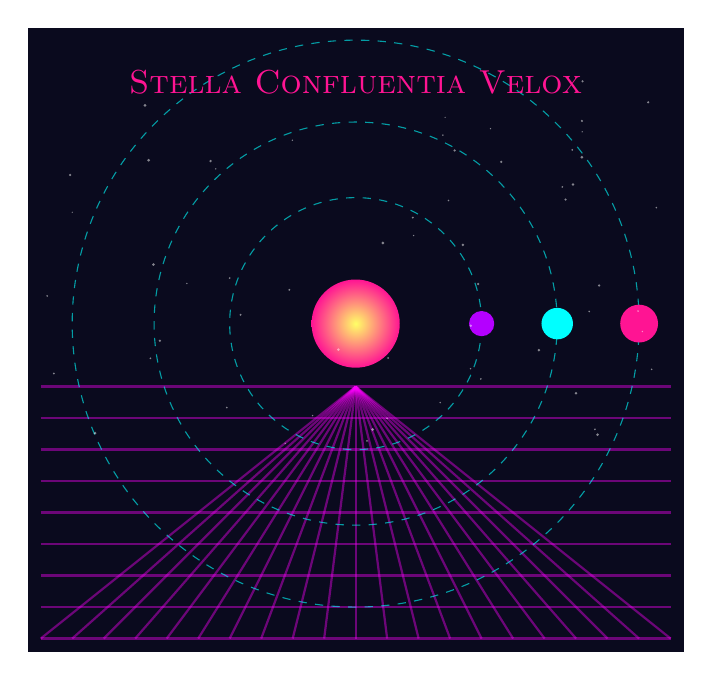
\begin{tikzpicture}[scale=0.8, background rectangle/.style={fill=spaceblack}, show background rectangle]

% Retro grid on bottom
\begin{scope}[shift={(-5,-5)}]
  \foreach \x in {0,0.5,...,10} {
    \draw[neongrid, opacity=0.4, thick] (\x,0) -- (5,4);
  }
  \foreach \y in {0,0.5,...,4} {
    \draw[neongrid, opacity=0.4, thick] (0,\y) -- (10,\y);
  }
\end{scope}


% Star (sun) with glow
\shade[inner color=neonyellow, outer color=neonpink] (0,0) circle (0.7);

% Orbits
\foreach \r in {2, 3.2, 4.5} {
  \draw[neonblue, thin, dashed, opacity=0.6] (0,0) circle (\r);
}

% Planets
\filldraw[fill=neonpurple, draw=none] (2,0) circle (0.2);
\filldraw[fill=neonblue, draw=none] (3.2,0) circle (0.25);
\filldraw[fill=neonpink, draw=none] (4.5,0) circle (0.3);

% Stars
\foreach \i in {1,...,60} {
  \pgfmathsetmacro{\x}{rnd*10 - 5}
  \pgfmathsetmacro{\y}{rnd*6 - 2}
  \fill[white, opacity=0.5] (\x,\y) circle (0.01 + rnd*0.015);
}

% Adding the name "Systema Solare Transitus"
\node[neonpink, above] at (0,3.5) {\large \textsc{Stella Confluentia Velox}};

\end{tikzpicture}
\end{center}

\end{frame}

%%

\begin{frame}{Markov chain coupling}
\begin{itemize}
    \item Markov chain coupling is one of the most important techniques for proving fast mixing.

    \bigskip
    \item Fast mixing means that $t_\mathrm{mix}$ scales poly-logarithmically in $|\Omega|$.

    \bigskip
    \item Markov chain couplings are at the heart of our novel quantization method.
\end{itemize}    
\end{frame}

%%

\begin{frame}{Drunk Eve in Manhattan}

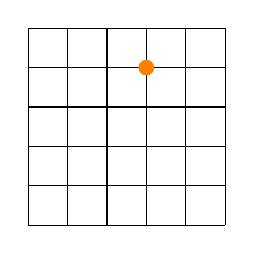
\begin{tikzpicture}[scale=0.5]
    % Draw the grid
    \draw[step=1cm,black,thin] (0,0) grid (5,5);

    % Place a red circle at position (2,3)
    \fill[orange] (3,4) circle (0.2);
\end{tikzpicture}

\begin{itemize}
\item Drunk \textcolor{orange}{Eve} moves randomly around Manhattan.

\item At each time step, Eve measures two $|+\>$ states in the computational basis.

\item The two bits determine whether Eve moves up, down, left, or right, but she cannot leave the grid.

\item Eve stays where she is if no move is possible.

\bigskip
\item The stationary distribution $\pi$ is approximately uniform (the effects due to the boundaries diminish as the size increases).
\end{itemize}
\end{frame}

%%

\begin{frame}{Drunk Alice and Bob in Manhattan}
    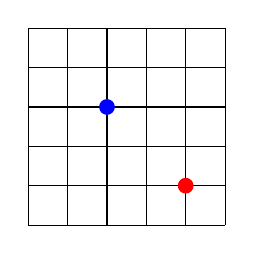
\begin{tikzpicture}[scale=0.5]
    % Draw the grid
    \draw[step=1cm,black,thin] (0,0) grid (5,5);

    % Place a red circle at position (2,3)
    \fill[blue] (2,3) circle (0.2);
    \fill[red] (4,1) circle (0.2);
\end{tikzpicture}

\begin{itemize}
\item Drunk \textcolor{red}{Alice} and \textcolor{blue}{Bob} move randomly around Manhattan.

\item At each time step, Alice and Bob measure the halves of two Bell states $|\Phi^+\>=\tfrac{1}{\sqrt{2}}(|00\>+|11\>)$ shared between them.

\item The rules for moving are the same as in the Eve example.

\bigskip
\item Viewed individually, they move like Eve.

\item It's also easy to see that eventually Alice and Bob will find each other.

\item Once Alice and Bob meet, they stay together forever.

\end{itemize}
\end{frame}

%%

\begin{frame}{Formal definition of Markov chain coupling}
A coupling is a Markov chain on state space $\Omega\times\Omega$ with transition matrix $C =(c_{(x',y'), (x,y)})$ so that:

\medskip
\begin{enumerate}
    \item Each component viewed separately undergoes transitions according to the original transition matrix $P$:
    %
    \begin{align*}
        \sum_{y'} c_{(x',y'),(x,y)} 
        &= 
        p_{x',x} \\
        \sum_{x'} c_{(x',y'),(x,y)} 
        &= 
        p_{y',y}
    \end{align*}
    %    
    \item The two components remain together forever once they have met, that is, $x'=y'$ if $x=y$:
    \begin{align*}
        c_{(x',x'),(x,x)}
        &=
        p_{x'x} \\
        c_{(x',y'),(x,x)} 
        &=
        0 \mbox{ for } x'\neq y'
    \end{align*}
    %
    \item The two components satisfy the symmetry condition:
    \begin{align*}
        c_{(x',y'),(x,y)} =
        c_{(y',x'),(y,x)}
    \end{align*}
\end{enumerate}
\end{frame}

%%

\begin{frame}{Connection between coalescence and mixing times I}

\begin{itemize}
\item Let $(X_m,Y_m)$ denote the random state of the coupling that starts in the initial state $(x,y)$ and makes $m$ transitions according to the transition matrix $C$. 

\bigskip
\item Let $\tau_\mathrm{coal}$ denote the random variable  
\begin{align*}
    \tau_\mathrm{coal} 
    &=
    \min\{ m : X_\ell = Y_\ell \mbox{ for all } \ell \ge m\},
\end{align*}
which is called the coalescence time for the initial state $(x,y)$.
\end{itemize}
\end{frame}

%%

\begin{frame}{Connection between coalescence and mixing times II}

\begin{itemize}
\item The total variation distance $d(m)$ and the mixing time $t_\mathrm{mix}$ are bounded from above by
\begin{align*}
    d(m) 
    &\le 
    \max_{x,y} \Pr_{x,y}\big(\tau_\mathrm{coal} > m \big) \\
    t_\mathrm{mix} 
    &\le 
    4 \max_{x,y} \mathbb{E}_{x,y}(\tau_\mathrm{coal}).
\end{align*}

\medskip
\item Thus, the problem of showing that the Markov chain with transition matrix $P$ mixes fast reduces to the problem of constructing a suitable coupling with transition matrix $C$ that coalesces quickly when starting in any initial state $(x,y)$.

\medskip
\item See \emph{Markov Chains and Mixing Times} by David A.~Levin and Yuval Peres, 2nd edition.

\end{itemize}
\end{frame}

%%

\begin{frame}{Coupling time}

\begin{itemize}
    \item In analogy to the mixing time $t_\mathrm{mix}$, it is convenient for our analysis to introduce the coupling time $t_\mathrm{couple}$.

    \bigskip
    \item We define it as
    \begin{align*}
        t_\mathrm{couple}
        &=
        \min \left\{ 
            m : 
            \max_{x, y} \Pr_{x,y}( \tau_{\mathrm{coal}} > m ) \le \frac{1}{4}
        \right\}.
    \end{align*}
\end{itemize}
\end{frame}

%%

\begin{frame}{Stellar Scale Research Intuition}
\begin{itemize}
    \item Using quantum notation, we can express the transition matrix $C=(c_{(x',y'),(x,y)})\in\cL(\C^N \otimes \C^N)$ as
    \begin{align*}
        C 
        &=
        \sum_{x',y',x,y\in\Omega} c_{(x',y'),(x,y)} 
        (|x'\> \otimes |y'\>)\,(\<x| \otimes \<y|). 
    \end{align*}

    \medskip
    \item The classical map $C$ acts on ket vectors of the form $|x\> \otimes |y\>$ and maps them to convex combinations of ket vectors $|x'\> \otimes |y'\>$.

    \medskip
    \item In contrast, a quantum map $\cE\in\cL(\C^{N\times N})$ must act on outer products of the form $|x\>\<y|$ and map them to linear combinations of outer products $|x'\>\<y'|$.

    \medskip
    \item Question: How can we cook up a useful quantum map $\cT$ based on the transition matrix $C$?
\end{itemize}
    
\end{frame}

%%

\iffalse

\begin{frame}{Quantum map I}

\begin{itemize}
    \item $\cT$ is completely positive. 

    \medskip
    It preserves the positivity of the density matrix for any larger system.
    \begin{align*}
        \text{Positive Map: } & \cT(\rho) \geq 0 \text{ for } \rho \geq 0 \\
        & \\
        \text{Completely Positive Map: } & (\cT \otimes I_d)(\sigma) \geq 0 \text{ for } \sigma \ge 0
    \end{align*}

    \bigskip
    \item $\cT$ is trace-preserving. 

    \medskip
    The trace of the density matrix remains unchanged after the map is applied, ensuring the total probability sums to $1$.
    \begin{align*}
        \text{Trace-Preserving: } \text{Tr}[\cT(\rho)] = \text{Tr}[\rho]
    \end{align*}

\end{itemize}

\end{frame}

%%

\begin{frame}{Quantum map II}
\begin{itemize}
    \item A quantum map $\cT$ has a Kraus representation:
    \begin{align*}
        \cT(\rho) = \sum_r A_r \rho A_r^\dagger, \quad \sum_r A_r^\dagger A_r = I
    \end{align*}

    \item Schr\"odinger picture: $\cT$ describes how states $\rho$ evolve.

    \medskip
    \item Heisenberg picture: the dual map $\cT^*$ describes how observable $M$ evolve
    \begin{align*}
        \cT^*(M) 
        &=
        \sum_{r} A_r^\dagger M A_r.
    \end{align*}

    \item We have
    \begin{align*}
        \tr[ M \, \cT(\rho)]
        &=
        \tr[ \cT^*(M) \, \rho].
    \end{align*}
\end{itemize}
\end{frame}

\fi

%%

\begin{frame}{Stellar Scale Research Summary I}
\begin{itemize}

\item Let $C=(c_{(x',y'),(x,y)})$ be the transition matrix of an arbitrary coupling of an ergodic Markov chain with transition matrix $P=(p_{x',x})$ and stationary distribution $\pi=(\pi_x)$.

\bigskip
\item Define
\begin{align*}
    \cT^*(\bullet) 
    &= 
    D^{-1/2} \cC^*( D^{1/2} \bullet D^{1/2} ) D^{-1/2} \quad\quad \mbox{where} \\
    & \\
    \cC^*(\bullet)
    &=
    \sum_{x,y,x',y' \in \Omega} c_{(x',y'),(x,y)} \,
    |x'\>\<x| \bullet |y\>\<y'| \\
    D
    &=
    \mathrm{diag}(\pi_x : x \in \Omega).
\end{align*}

\item The quantized coupling $\cT$ is defined as the dual of the linear map $\cT^*$ with respect to the Hilbert-Schmidt inner product.
\end{itemize}
\end{frame}

%%

\begin{frame}{Stellar Scale Research Summary II}

\begin{itemize}
\item Let $C$ be any coupling.

\bigskip
\item The quantized coupling $\cT$ is trace preserving.

\bigskip
\item The quantized coupling $\cT$ has $|\sqrt{\pi}\>\<\sqrt{\pi}|$ as fixed point.

\end{itemize}
\end{frame}

%%

\begin{frame}{Stellar Scale Research Summary III}

\begin{itemize}
\item Assume that $C$ satisfies certain additional conditions so that the corresponding $\cT$ is also completely positive.

\medskip
\item Then, given any initial state $\rho$, the quantized coupling $\cT$ converges to the qsample $|\sqrt{\pi}\>\<\sqrt{\pi}|$ in trace norm distance as
\begin{align*}
    \frac{1}{2} \big\| \cT^m(\rho) - |\sqrt{\pi}\>\<\sqrt{\pi} \big\|_\mathrm{tr}
    &\le 
    \sqrt{\varepsilon}
\end{align*}
after 
\begin{align*}
    m 
    &\ge 
    \frac{1}{2}\log_2 \left( 
    \frac{1}{\varepsilon \, \pi_*}
    \right) \, t_\mathrm{couple}
\end{align*}
steps, where $\pi_*=\min\{\pi_x : x \in \Omega\}$.
\end{itemize}
\end{frame}

%%

\begin{frame}{Stellar Scale Research Summary IV}
\begin{itemize}
\item For independent and grand couplings, the resulting quantized coupling $\cT$ is completely positive.

\bigskip
\item The quantized coupling $\cT$ can be implemented efficiently for sparse grand couplings. 
\end{itemize}
\end{frame}

%%%%%%%%%%%%%%%%%%%%%%%%%%%%%%%%%%%%%%%%%%%%%%%%%%%


\begin{frame}{Planetary Scale Research Description}

\begin{center}

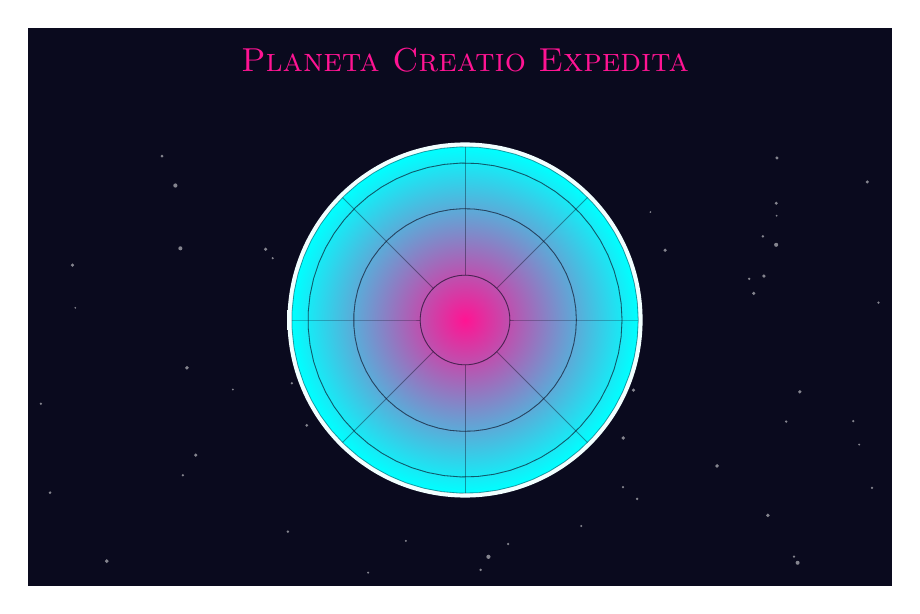
\begin{tikzpicture}[scale=1.1, background rectangle/.style={fill=spaceblack}, show background rectangle]

\begin{scope}[shift={(0,0)}]
% Stars
\foreach \i in {1,...,60} {
  \pgfmathsetmacro{\x}{rnd*10 - 5}
  \pgfmathsetmacro{\y}{rnd*5 - 3}
  \fill[white, opacity=0.5] (\x,\y) circle (0.01 + rnd*0.015);
}

% Atmosphere glow (drawn FIRST)
\shade[inner color=neonblue!30, outer color=neonblue!5]
  (0,0) circle (2.05);

% Planet (ocean)
\shade[inner color=neonpink, outer color=neonblue]
  (0,0) circle (2.0);

% Grid lines (longitude) - simplified
  \foreach \angle in {-75,-50,...,75} {
    \draw[spaceblack, opacity=0.4, line width=0.3pt] 
      plot[domain=0:360, samples=60] 
      ({2.0*cos(\x)*cos(\angle)}, {2.0*sin(\x)*cos(\angle)});
  }
  
  % Grid lines (latitude) - simplified
  \foreach \angle in {0,45,...,315} {
    \draw[spaceblack, opacity=0.4, line width=0.3pt] 
      plot[domain=-75:75, samples=60] 
      ({2.0*cos(\angle)*cos(\x)}, {2.0*sin(\angle)*cos(\x)});
  }
  
\node[text=neonpink] at (0,3) {\large \textsc{Planeta Creatio Expedita}};


\end{scope}
\end{tikzpicture}
\end{center}

\end{frame}

%%

\begin{frame}{Proof of fixed point I}
\begin{itemize}
    \item The qsample $|\sqrt{\pi}\>$ is a fixed point of the quantized coupling $\cT$, i.e., 
    \begin{align*}
        \cT(|\sqrt{\pi}\>\<\sqrt{\pi}|)
        &=
        |\sqrt{\pi}\>\<\sqrt{\pi}|.
    \end{align*}
\end{itemize}
\end{frame}

%%

\begin{frame}{Proof of fixed point II}
\begin{itemize}
    \item Recall that the matrix $D$ is given by
    \begin{align*}
        D=\mathrm{diag}(\pi_x : x \in \Omega).
    \end{align*}.

    \item We write the qsamples $|\sqrt{\pi}\>$ as
    \begin{align*}
    |\sqrt{\pi}\>
    &=
    \sum_{x \in \Omega} \sqrt{\pi_x} |x\> \\
    &=
    D^{1/2}|e\>
    \end{align*}
    where 
    \begin{align*}
        |e\>
        &=
        \sum_{x\in\Omega}|x\> =
        (1,1,\ldots,1)^T
    \end{align*} 
    is the all-ones vector.
\end{itemize}
\end{frame}

%%

\begin{frame}{Proof of fixed point III}
    
\begin{itemize}
    \item We have 
    \begin{align*}
        \cC(|e\>\<e|)
        &=
        \sum_{x,y,x',y'\in\Omega} c_{(x',y'),(x,y)} |y\>\<y'|e\>\<e|x'\>\<x| \\
        &=
        \sum_{x,y,x',y'\in\Omega} c_{(x',y'),(x,y)} |y\>\<x| \\
        &=
        \sum_{y,x} |y\>\<x| \\
        &= |e\>\<e|,
    \end{align*}
    since $C=(c_{(x',y'),(x,y)})$ is column stochastic.
    \end{itemize}
\end{frame}

%%

\begin{frame}{Proof of fixed point IV}
\begin{itemize}
    \item Inserting $|\sqrt{\pi}\>\<\sqrt{\pi}|$ into
    \begin{align*}
        \cT(\bullet) 
        &=
        D^{1/2} \, \cC( D^{-1/2} \bullet D^{-1/2}) \, D^{1/2}
    \end{align*}
    yields 
    \begin{align*}
        \cT(|\sqrt{\pi}\>\<\sqrt{\pi}|)
        &=
        D^{1/2} \, \cC( D^{-1/2} |\sqrt{\pi}\>\<\sqrt{\pi}| D^{-1/2} ) \, D^{1/2} \\
        &=
        D^{1/2} \, \cC(|e\>\<e|) \, D^{1/2} \\
        &=
        D^{1/2} |e\>\<e| D^{1/2} \\
        &= 
        |\sqrt{\pi}\>\<\sqrt{\pi}|.
    \end{align*}
\end{itemize}
\end{frame}


%%

\begin{frame}{Sketch of convergence proof I}
\begin{itemize}
    \item Let $Q=|\sqrt{\pi}\>\<\sqrt{\pi}|$ and $Q^\perp = I - Q$.

    \medskip
    \item Assume we can find an integer $m$ for some $\varepsilon>0$ so that 
    \begin{align*}
        \tr[Q^\perp \cT^m(\rho)]
        &\le
        \varepsilon
    \end{align*} for all initial states $\rho$.

    \medskip
    \item Then, we have
    \begin{align*}
        \| \cT^k(\rho) - |\sqrt{\pi}\>\<\sqrt{\pi}| \|_\mathrm{tr} \le 2 \sqrt{\varepsilon}
    \end{align*}
    for all $k\ge m$.

    \medskip
    \item The proof of this technical result relies on some fundamental tools in quantum information processing, such as the gentle measurement lemma and the data processing inequality.
\end{itemize}
\end{frame}

%%

\begin{frame}{Sketch of convergence proof II}
\begin{itemize}
    \item We have
    \begin{align*}
        \tr[Q^\perp \cT^m(\rho)]
        &=
        \tr[(\cT^*)^m (Q^\perp) \, \rho] \\
        &\le
        \tr[(\cT^*)^m (Q^\perp)] \\
        &=
        \tr[D^{-1/2} (\cC^*)^m (D^{1/2} Q^\perp D^{1/2}) D^{-1/2} ] \\
        &\le
        \frac{1}{\pi_*} \tr[(\cC^*)^m (D^{1/2} Q^\perp D^{1/2})]
    \end{align*}
    where $\pi_*=\min\{ \pi_x  : x \in \Omega\}$.
\end{itemize}
\end{frame}

%%

\begin{frame}{Sketch of convergence proof III}
\begin{itemize}
    \item Moreover, we show that 

    \medskip
    \begin{itemize}
        \item the rescaled projector $D^{1/2} Q^\perp D^{1/2}$ can be written as a convex combination of ``quasi-particles'' corresponding to elementary graph Laplacians 
        \begin{align*}
            \rho_{x,y} 
            &=
            |-_{x,y}\>\<-_{x,y}|
        \end{align*} 
        where $|-_{x,y}\>=\frac{1}{\sqrt{2}}(|x\>-|y\>)$.

        \medskip
        \item the map $\cC^*$ scatters $\rho_{x,y}$ into sub-stochastic combinations according to
        \begin{align*}
            \cC^*(\rho_{x,y})
            &=
            \sum_{x',y'} c_{(x',y'),(x,y)} \rho_{x',y'}.
        \end{align*}

        \medskip
        \item the power $(\cC^*)^m$ annihilates the quasi-particle $\rho_{x,y}$ whenever $C^m$ coalesces $(x,y)$. 
    \end{itemize}
\end{itemize}
\end{frame}

%%

\begin{frame}{Grand couplings}
\begin{itemize}
    \item A random mapping representation of the transition matrix $P=(p_{x',x})$ on state space $\Omega$ is a function $f : \Omega \times \cR \rightarrow \Omega$, along with a $\cR$-valued random variable $R$, satisfying
    \begin{align*}
        \Pr(f(x,R)=x') = p_{x',x}
    \end{align*}
    for all possible pairs of current state $x$ and successor state $x'$.

    \medskip
    \item The transition matrix $P$ can be expressed as
    \begin{align*}
        P 
        &= \sum_{r\in\cR} \sum_{x\in\Omega} \Pr(r) |f(x,r)\>\<x|.
    \end{align*}

    \medskip
    \item The transition matrix $C_\mathrm{grand}$ of the corresponding grand coupling can be expressed as
    \begin{align*}
        C_\mathrm{grand} 
        &=
        \sum_{r\in\cR} \sum_{x,y\in\Omega} \Pr(r) (|f(x,r)\> \otimes |f(y,r)\>) \, (\<x| \otimes \<y|)
    \end{align*}
\end{itemize}
    
\end{frame}

%%

\begin{frame}{Example of grand coupling -- random colorings I}
\begin{itemize}
    \item Let $G=(V,E)$ be a graph with vertex set $V$ and edge set $E$. 

    \medskip
    \item A proper $q$-coloring of $G$ is an element $x$ of $\{1,\ldots,q\}^V$, the set of functions from $V$ to $\{1,\ldots,q\}$, such that $x(v)\neq x(w)$ for all edges $\{v,w\}\in E$.

\medskip
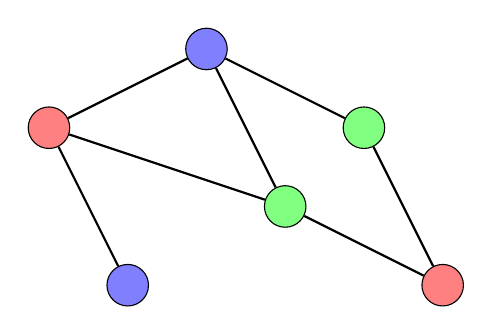
\begin{tikzpicture}[
    vertex/.style={circle, draw, minimum size=1.5em},
    edge/.style={thick, -}
]

% Define vertices
\node[vertex, fill=red!50] (v1) at (0, 2) {};
\node[vertex, fill=blue!50] (v2) at (2, 3) {};
\node[vertex, fill=green!50] (v3) at (4, 2) {};
\node[vertex, fill=blue!50] (v4) at (1, 0) {};
\node[vertex, fill=green!50] (v5) at (3, 1) {};
\node[vertex, fill=red!50] (v6) at (5, 0) {};

% Define edges
\draw[edge] (v1) -- (v2);
\draw[edge] (v1) -- (v4);
\draw[edge] (v2) -- (v3);
\draw[edge] (v2) -- (v5);
\draw[edge] (v3) -- (v6);
\draw[edge] (v1) -- (v5);
\draw[edge] (v5) -- (v6);

\end{tikzpicture}

\end{itemize}
\end{frame}

%%

\begin{frame}{Example of grand coupling -- random colorings II}
\begin{itemize}
    \item Let $\cX$ denote the collection of all proper $q$-colorings of $G$ and $\pi$ denote the uniform distribution of on $\cX$.

    \medskip
    \item A Metropolis chain for $\pi$ can be constructed as follows:

    \medskip
    \begin{itemize}
        \item select a vertex $v\in V$ uniformly and then select a color $k\in\{1,\ldots,q\}$ uniformly. 

        \medskip
        \item if $k$ is allowable at $v$, then vertex $v$ is assigned the color $k$; otherwise, no transition is made.
    \end{itemize}

\end{itemize}
\end{frame}

%%

\begin{frame}{Example of grand coupling -- random colorings III}
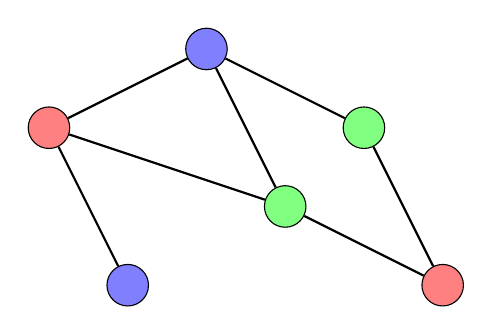
\begin{tikzpicture}[
    vertex/.style={circle, draw, minimum size=1.5em},
    edge/.style={thick, -}
]

% Define vertices
\node[vertex, fill=red!50] (v1) at (0, 2) {};
\node[vertex, fill=blue!50] (v2) at (2, 3) {};
\node[vertex, fill=green!50] (v3) at (4, 2) {};
\node[vertex, fill=blue!50] (v4) at (1, 0) {};
\node[vertex, fill=green!50,] (v5) at (3, 1) {};
\node[vertex, fill=red!50] (v6) at (5, 0) {};

% Define edges
\draw[edge] (v1) -- (v2);
\draw[edge] (v1) -- (v4);
\draw[edge] (v2) -- (v3);
\draw[edge] (v2) -- (v5);
\draw[edge] (v3) -- (v6);
\draw[edge] (v1) -- (v5);
\draw[edge] (v5) -- (v6);

\end{tikzpicture}

%%

\medskip
select $v$ to be the center node, and $k$ to be yellow

\medskip
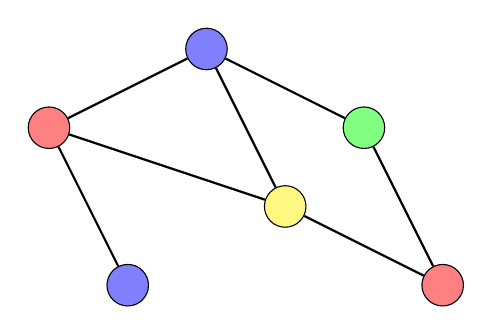
\begin{tikzpicture}[
    vertex/.style={circle, draw, minimum size=1.5em},
    edge/.style={thick, -}
]

% Define vertices
\node[vertex, fill=red!50] (v1) at (0, 2) {};
\node[vertex, fill=blue!50] (v2) at (2, 3) {};
\node[vertex, fill=green!50] (v3) at (4, 2) {};
\node[vertex, fill=blue!50] (v4) at (1, 0) {};
\node[vertex, fill=yellow!50] (v5) at (3, 1) {};
\node[vertex, fill=red!50] (v6) at (5, 0) {};

% Define edges
\draw[edge] (v1) -- (v2);
\draw[edge] (v1) -- (v4);
\draw[edge] (v2) -- (v3);
\draw[edge] (v2) -- (v5);
\draw[edge] (v3) -- (v6);
\draw[edge] (v1) -- (v5);
\draw[edge] (v5) -- (v6);

\end{tikzpicture}

\end{frame}

%%

\begin{frame}{Example of grand coupling -- random colorings IV}
\begin{itemize}
    \item A grand coupling also generates such $(v,k)$ uniformly and applies the corresponding recoloring update to both components.

    \medskip
    \item The bound
    \begin{align*}
        \Pr_{x,y}\{\tau_\mathrm{coal} > m\} 
        &\le
        n \exp\big( - m \, c_\mathrm{met}(\Delta, q) / n\big), 
    \end{align*}
    holds for all pairs of initial $q$-colorings $x$ and $y$. 
    
    \medskip
    $\Delta$ denotes the maximum degree and $c_\mathrm{met}=1 - (3\Delta) / q$.  
\end{itemize}
\end{frame}

%%

\begin{frame}{Implementation I}
\begin{itemize}
\item Assume that we have a random mapping representation such that
\begin{itemize}
    \item we can efficiently compute the images and pre-images of the function $f : \Omega \times \cR \rightarrow \Omega$

    \medskip
    \item we can efficiently compute the probabilities $\Pr(r)$
    
    \medskip
    \item we can efficiently compute the ratios $\pi(x)/\pi(y)$ for the stationary distribution. 
\end{itemize}

\medskip
\item Then, the Kraus operators
\begin{align*}
    A_r 
    &= 
    \sqrt{\Pr(r)} \sum_{x\in\Omega} D^{1/2} |x\>\<f(x,r)| D^{-1/2}.
\end{align*}
of the quantized coupling $\cT$ are $|\cR|$-sparse. 

\end{itemize} 
\end{frame}

%%

\begin{frame}{Implementation II}
\begin{itemize}
    \item We can efficiently construct block-encodings of the sparse matrices $A_r$, i.e., unitaries $U_r$ of the form
\end{itemize}
    \begin{align*}
        U_r
        &=
        \left(
        \begin{array}{cc}
            A_r & C_r \\
            B_r & D_r
        \end{array}
        \right) \\
        &=
        |0\>\<0| \otimes A_r +
        |0\>\<1| \otimes B_r +
        |1\>\<0| \otimes C_r +
        |1\>\<1| \otimes D_r.
    \end{align*}

\begin{itemize}
    \item We can also efficiently implement the controlled unitary
    \begin{align*}
        W 
        &=
        \sum_{r\in\cR} |r\>\<r| \otimes U_r.
    \end{align*}

\end{itemize}
\end{frame}

%%

\begin{frame}{Implementation III}
\begin{itemize}
    \item Given any initial state $|\xi\>$, we can use $W$ to prepare
    \begin{align*}
        \frac{1}{\sqrt{|\cR|}} 
        \sum_{r\in\cR}
        |r\> \otimes 
        (|0\> \otimes A_r|\xi\> + |1\> \otimes B_r|\xi\>) 
    \end{align*}

    \medskip
    \item We now leverage oblivious amplitude amplification to prepare
    \begin{align*}
        \sum_{r\in\cR} |r\> \otimes |0\> \otimes A_r|\xi\> 
    \end{align*}

    \item Tracing out the first two registers yields
    \begin{align*}
        \cT(|\xi\>\<\xi|)
        &=
        \sum_{r\in\cR} A_r |\xi\>\<\xi| A_r^\dagger
    \end{align*}

    \medskip
    \item This shows that $\cT$ can be implemented efficiently since the above arguments hold for arbitrary $|\xi\>$.
\end{itemize}
\end{frame}

%%

\begin{frame}{Some open problems}
\begin{itemize}
    \item Improve analysis of convergence.

    \medskip
    For instance, can we avoid the factor $1/\pi_*$?

    \bigskip
    \item Generalize to the quantum setting.

    \medskip
    Given a fast mixing quantum channel $\mathcal{E}$ with fixed point $\sigma$, can we design a quantum channel $\mathcal{E}_\mathrm{pure}$ that 
    
    \medskip
    \begin{itemize}
    \item[(i)] has the purification
    \begin{align*}
        (\sqrt{\sigma} \otimes I) |\Phi\>
    \end{align*}
    as fixed point and

    \medskip
    \item[(ii)] converges to it quickly?
    \end{itemize}
\end{itemize}
\end{frame}

%%

\begin{frame}{Thank you for your attention!}

\end{frame}

\end{document}